%% LaTeX2e class for student theses
%% thesis.tex
%% 
%% Karlsruhe Institute of Technology
%% Institute for Program Structures and Data Organization
%% Chair for Software Design and Quality (SDQ)
%%
%% Dr.-Ing. Erik Burger
%% burger@kit.edu
%%
%% See https://sdqweb.ipd.kit.edu/wiki/Dokumentvorlagen
%%
%% Version 1.3.5, 2020-06-26

%% Available page modes: oneside, twoside
%% Available languages: english, ngerman
%% Available modes: draft, final (see README)
\documentclass[twoside, english]{sdqthesis}

\usepackage{float}

% add support for quotes
\let\oldquote\quote
\let\endoldquote\endquote
\renewenvironment{quote}[2][]
  {\if\relax\detokenize{#1}\relax
     \def\quoteauthor{#2}%
   \else
     \def\quoteauthor{#2~---~#1}%
   \fi
   \oldquote}
  {\par\nobreak\smallskip\hfill(\quoteauthor)%
   \endoldquote\addvspace{\bigskipamount}}

% set colors for links, urls and citations
\hypersetup{colorlinks,linkcolor={blue},citecolor={blue},urlcolor={blue}}  
% new paragraph should not indent but add a blank line!
\usepackage[parfill]{parskip}

% for the use of align
\usepackage{amsmath}

% Print code in latex:
\usepackage{xcolor}

\definecolor{commentsColor}{rgb}{0.497495, 0.497587, 0.497464}
\definecolor{keywordsColor}{rgb}{0.000000, 0.000000, 0.635294}
\definecolor{stringColor}{rgb}{0.558215, 0.000000, 0.135316}

\usepackage{pdfpages}

\usepackage{listings}
\lstset{ %
  backgroundcolor=\color{white},   % choose the background color; you must add \usepackage{color} or \usepackage{xcolor}
  basicstyle=\footnotesize,        % the size of the fonts that are used for the code
  breakatwhitespace=false,         % sets if automatic breaks should only happen at whitespace
  breaklines=true,                 % sets automatic line breaking
  captionpos=b,                    % sets the caption-position to bottom
  commentstyle=\color{commentsColor}\textit,    % comment style
  deletekeywords={...},            % if you want to delete keywords from the given language
  escapeinside={\%*}{*)},          % if you want to add LaTeX within your code
  extendedchars=true,              % lets you use non-ASCII characters; for 8-bits encodings only, does not work with UTF-8
  frame=tb,	                   	   % adds a frame around the code
  keepspaces=true,                 % keeps spaces in text, useful for keeping indentation of code (possibly needs columns=flexible)
  keywordstyle=\color{keywordsColor}\bfseries,       % keyword style
  language=Python,                 % the language of the code (can be overrided per snippet)
  otherkeywords={*,...},           % if you want to add more keywords to the set
  numbers=left,                    % where to put the line-numbers; possible values are (none, left, right)
  numbersep=5pt,                   % how far the line-numbers are from the code
  numberstyle=\tiny\color{commentsColor}, % the style that is used for the line-numbers
  rulecolor=\color{black},         % if not set, the frame-color may be changed on line-breaks within not-black text (e.g. comments (green here))
  showspaces=false,                % show spaces everywhere adding particular underscores; it overrides 'showstringspaces'
  showstringspaces=false,          % underline spaces within strings only
  showtabs=false,                  % show tabs within strings adding particular underscores
  stepnumber=1,                    % the step between two line-numbers. If it's 1, each line will be numbered
  stringstyle=\color{stringColor}, % string literal style
  tabsize=2,	                   % sets default tabsize to 2 spaces
  title=\lstname,                  % show the filename of files included with \lstinputlisting; also try caption instead of title
  columns=fixed                    % Using fixed column width (for e.g. nice alignment)
}

%% ---------------------------------
%% | Information about the thesis  |
%% ---------------------------------

%% Name of the author
\author{Philipp Weinmann}

%% Title (and possibly subtitle) of the thesis
\title{Tuning of Explainable Artificial Intelligence (XAI) tools in the field of text analysis}

%% Type of the thesis 
\thesistype{Bachelor's Thesis}

%% Change the institute here, ``IPD'' is default
% \myinstitute{Institute for \dots}

%% You can put a logo in the ``logos'' directory and include it here
%% instead of the SDQ logo
% \grouplogo{myfile}
%% Alternatively, you can disable the group logo
% \nogrouplogo

%% The reviewers are the professors that grade your thesis
\reviewerone{Prof. Dr.-Ing. Klemens Böhm}
\reviewertwo{Prof. Dr. Pascal Friederich}

%% The advisors are PhDs or Postdocs
\advisorone{M.Sc. Clemens Müssener}
%% The second advisor can be omitted
%% \advisortwo{M.Sc. D}

%% Please enter the start end end time of your thesis
\editingtime{15. January 2021}{17. June 2021}

\settitle

%% --------------------------------
%% | Settings for word separation |
%% --------------------------------

%% Describe separation hints here.
%% For more details, see 
%% http://en.wikibooks.org/wiki/LaTeX/Text_Formatting#Hyphenation
\hyphenation{
% me-ta-mo-del
}

%% --------------------------------
%% | Bibliography                 |
%% --------------------------------

%% Use biber instead of BibTeX, see README
\usepackage[citestyle=numeric,style=numeric,backend=biber, sorting=none]{biblatex}
\addbibresource{thesis.bib}

%% ====================================
%% ====================================
%% ||                                ||
%% || Beginning of the main document ||
%% ||                                ||
%% ====================================
%% ====================================
\begin{document}

%% Set PDF metadata
\setpdf

%% Set the title
\maketitle

%% The Preamble begins here
\frontmatter

% declaration signed and scanned
 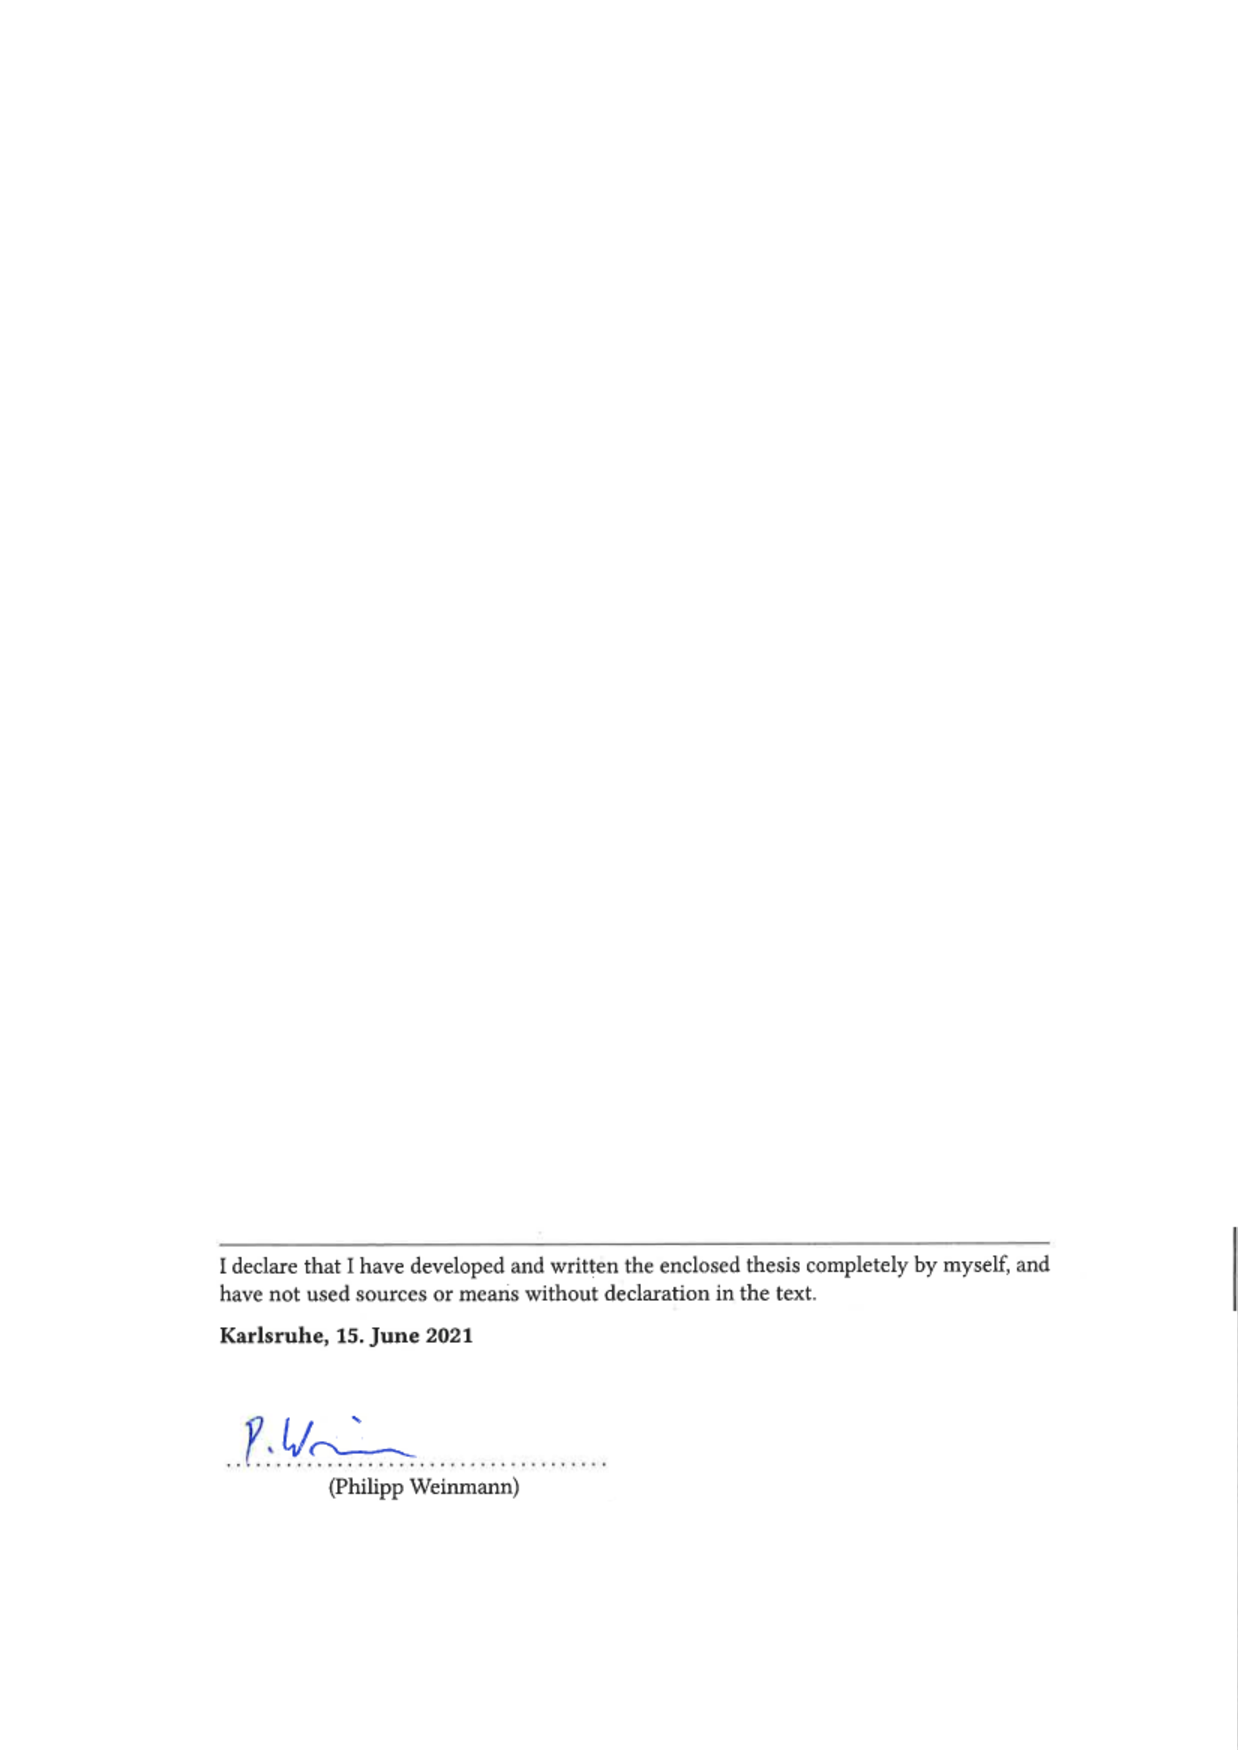
\includepdf[pages=-]{sections/Erklaerung_unterschrieben_weis.pdf}

%%% LaTeX2e class for student theses: Declaration of independent work
%% sections/declaration.tex
%% 
%% Karlsruhe Institute of Technology
%% Institute for Program Structures and Data Organization
%% Chair for Software Design and Quality (SDQ)
%%
%% Dr.-Ing. Erik Burger
%% burger@kit.edu
%%
%% Version 1.3.5, 2020-06-26

\thispagestyle{empty}
\null\vfill
\noindent\hbox to \textwidth{\hrulefill} 
\iflanguage{english}{I declare that I have developed and written the enclosed
thesis completely by myself, and have not used sources or means without
declaration in the text.}%
{Ich versichere wahrheitsgemäß, die Arbeit
selbstständig angefertigt, alle benutzten Hilfsmittel vollständig und genau
angegeben und alles kenntlich gemacht zu haben, was aus Arbeiten anderer
unverändert oder mit Änderungen entnommen wurde.}
 
 
%% ---------------------------------------------
%% | Replace PLACE and DATE with actual values |
%% ---------------------------------------------
\textbf{Karlsruhe, 15. June 2021}
\vspace{1.5cm}
 
\dotfill\hspace*{8.0cm}\\
\hspace*{2cm}(\theauthor) 
\cleardoublepage

\setcounter{page}{1}
\pagenumbering{roman}

%% ----------------
%% |   Abstract   |
%% ----------------
 
%% For theses written in English, an abstract both in English
%% and German is mandatory.
%%
%% For theses written in German, a German abstract is sufficient.
%%
%% The text is included from the following files:
%% - sections/abstract

\includeabstract

%% ------------------------
%% |   Table of Contents  |
%% ------------------------
\tableofcontents

\listoffigures
\listoftables

%% -----------------
%% |   Main part   |
%% -----------------

\mainmatter

\iffalse
\textcolor{red}{Feedback von Professoren: Framework und meine Ergebnisse könnten unabhängig voneinander betrachtet werden. Vielleicht in Part I und Part II aufteilen?? Des weiteren sollte related works in state of the art umbenannt werden und shap teil davon sein.}
\fi
%% LaTeX2e class for student theses
%% sections/content.tex
%% 
%% Karlsruhe Institute of Technology
%% Institute for Program Structures and Data Organization
%% Chair for Software Design and Quality (SDQ)
%%
%% Dr.-Ing. Erik Burger
%% burger@kit.edu
%%
%% Version 1.3.5, 2020-06-26

\chapter{Introduction}
\label{ch:Introduction}


\begin{quote}{Sundar Pichai}
\textit{AI is one of the most important things humanity is working on. It is more profound than [...] electricity or fire \cite{AIQuotePichai}}
\end{quote}

\section{Motivation}

\subsection{Need for explainable artificial intelligence in general}

Artificial Intelligence (AI) has been revolutionizing technology since computers were invented \cite{TimeLineOfAI}. For most of that time the limitation had been processing power, limiting the complexity of artificial intelligence. Therefore, except for the rare exception, artificial intelligence which was being run could be understood by reading the underlying code that defined it.


Past decades have seen tremendous increase in processing power (see \autoref{fig:topComp}) which has shifted the limitations of AI from computational to cognitive processing power.

\begin{figure}[H]
\centering
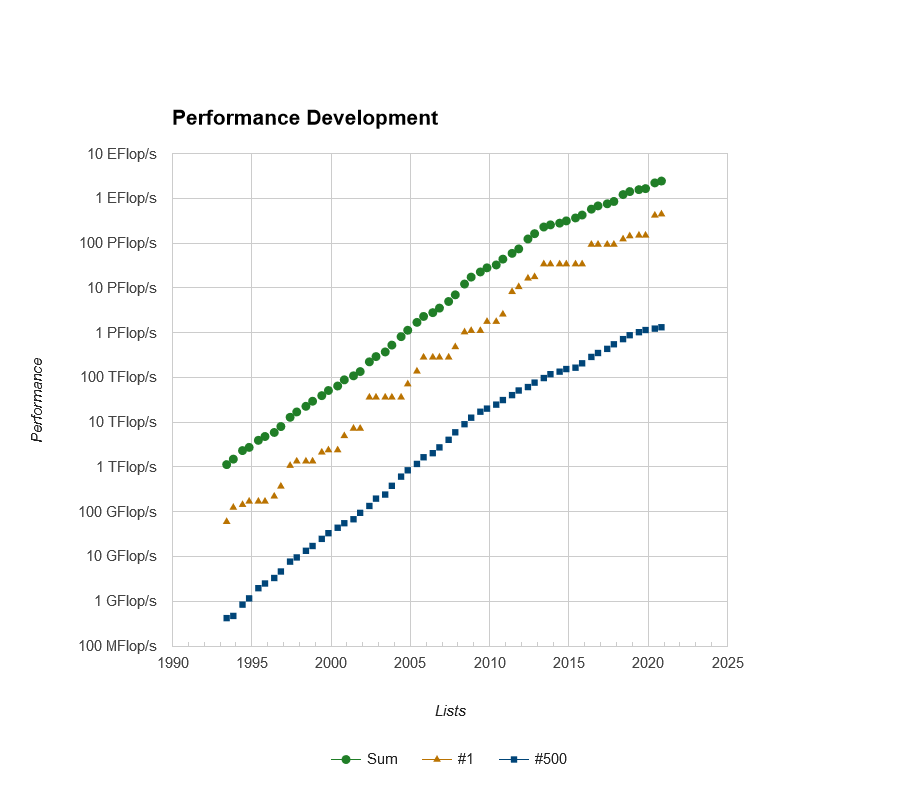
\includegraphics[width=\linewidth]{images/01_Intro/Top500.png}
\caption{Performance of the top 500 supercomputers over time \cite{top500}.}
\label{fig:topComp}
\end{figure}

This has culminated in the rise of a new type of algorithms, artificial neuronal networks. These apply a fundamentally different approach to AI. The human doesn't define the algorithm anymore but feeds data to a complex algorithm which writes its own program to solve a specific problem. These approaches have led to breakthroughs in many fields \cite{10.1145/3065386}. \par
While this step was arguably unavoidable for the advancement of AI, it poses its own challenges. Artificial neural networks can depend on millions of parameters \cite{szegedy2015going} which cannot, in their entirety, be understood due to our limited cognitive abilities. 

In \autoref{fig:complexity} I have tried to showcase the issue, modern day artificial neural networks are fundamentally more complex than any previous algorithms. 2013 is considered a breakthrough year in image recognition, with massive improvements in artificial neural network technology \cite{ILSVRC15}, but the exact moment the cognitive complexity barrier was breached is difficult to pinpoint.


\begin{figure}[H]
    \centering
    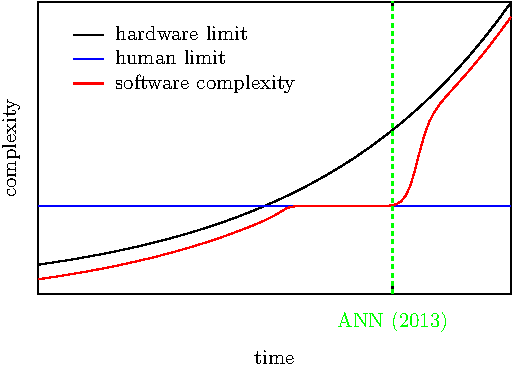
\includegraphics[width=0.8\linewidth]{images/01_Intro/Complexity.pdf}
    \caption{Breaking through the cognitive complexity barrier.}
    \label{fig:complexity}
\end{figure}

This inability to understand AI and algorithms in general poses a few fundamental problems.

\begin{itemize}
    \item How do we debug/improve algorithms we do not understand?
    \item How do we enforce laws on algorithms we do not understand?
    \item Can/should we use such an algorithm on applications where fatal errors are not permitted \textit{(ex: military applications)}
\end{itemize}



\subsection{Need for tools to analyse Explainable AI}

All of the above mentioned issues are being faced not only by scientists but more generally by software developers who do not have the luxury to spend months analysing one aspect of their software and require specialized tools to guide them. It can be argued that while neural networks where theorized decades ago, and could be implemented in hardware since the 2000s, it required frameworks and libraries like DistBelief, Tensorflow and more for their applications to become widespread and usable for most engineers and scientists. Theory and practicable tools need to go hand in hand to enable progress and in this context we wish to present our own framework to analyse explainable artificial intelligence tools.

\section{Applications for explainable AI}

The sceptical would argue that you cannot explain complex algorithms because they are by nature too complex to be understood in detail by a human. The argument would be, that if we were capable of explaining artificial neural networks, we could program them ourselves. While for certain cases this is true, it is not guaranteed. Multiple scenarios could happen:

\begin{enumerate}
    \item Developers just need a hint on how to solve a problem and an even incomplete explanation of a Neural Network enables them to code it in a humanly understandable way.
    \item We understand a fraction of how the artificial intelligence makes a decision but it is enough to disqualify it. This is especially important if some unwanted behaviour like biased \textit{(racist/sexist/...)} decisions are revealed.
    \item We understand a fraction of how the artificial intelligence makes a decision and the approach feels plausible to humans.
\end{enumerate}

Note that scenario three does not guarantee that no unwanted or even illegal behaviour is occurring. Similar to the quote from Edsger W. Dijkstra: \enquote{Program testing can be used to show the presence of bugs, but never to show their absence}, an incomplete explanation will never guarantee the absence of all issues opaque algorithms bring with them.
Nonetheless, XAI is fundamental if we wish to evaluate and compare algorithms with each other.


\section{Key questions}

In this bachelor thesis we will examine which approaches exist to understand artificial intelligence, meaning algorithms generated with the help of artificial neural networks, and we will explore one of these approaches in detail. In this context we will present a framework which has been developed by our team and myself to analyse XAI approaches and compare them with each other. Our key questions are which parameters are important for the usage of explainable artificial intelligence tools when applying them onto natural language in written form and how to tweak them to adjust unsatisfying explanations. Furthermore we will show how our framework can be used to create your own analysis.
\chapter{State or the art}
\label{ch:stateOfTheArt}

\section{Approaches to Explainable Artificial Intelligence}

There exist multiple approaches to XAI which each have their advantages and disadvantages. In this section we will briefly go over the most common ones \cite{XAIMethods}:
\begin{itemize}
    \item Perturbation based approaches.
    \item Function based approaches
    \item Surrogate-/ Sampling based approaches
    \item Structure-Based approaches
\end{itemize}

Each one of these takes a pretrained ANN and analyses it and its behaviour by analysing how its output depends on variations of the input.


Most advanced tools including Shap \cite{NIPS2017_7062} (the tool we used) combine several of these approaches trying to combine their respective advantages and compensating their respective disadvantages.

\subsection{Perturbation based approaches}

Perturbation based approaches excel in their simplicity. The core algorithmic logic is dependent on random or carefully chosen changes to features in the input data \cite{das2020opportunities}. This approach is best visualized when applied to images.

\begin{figure}[H]
    \centering
    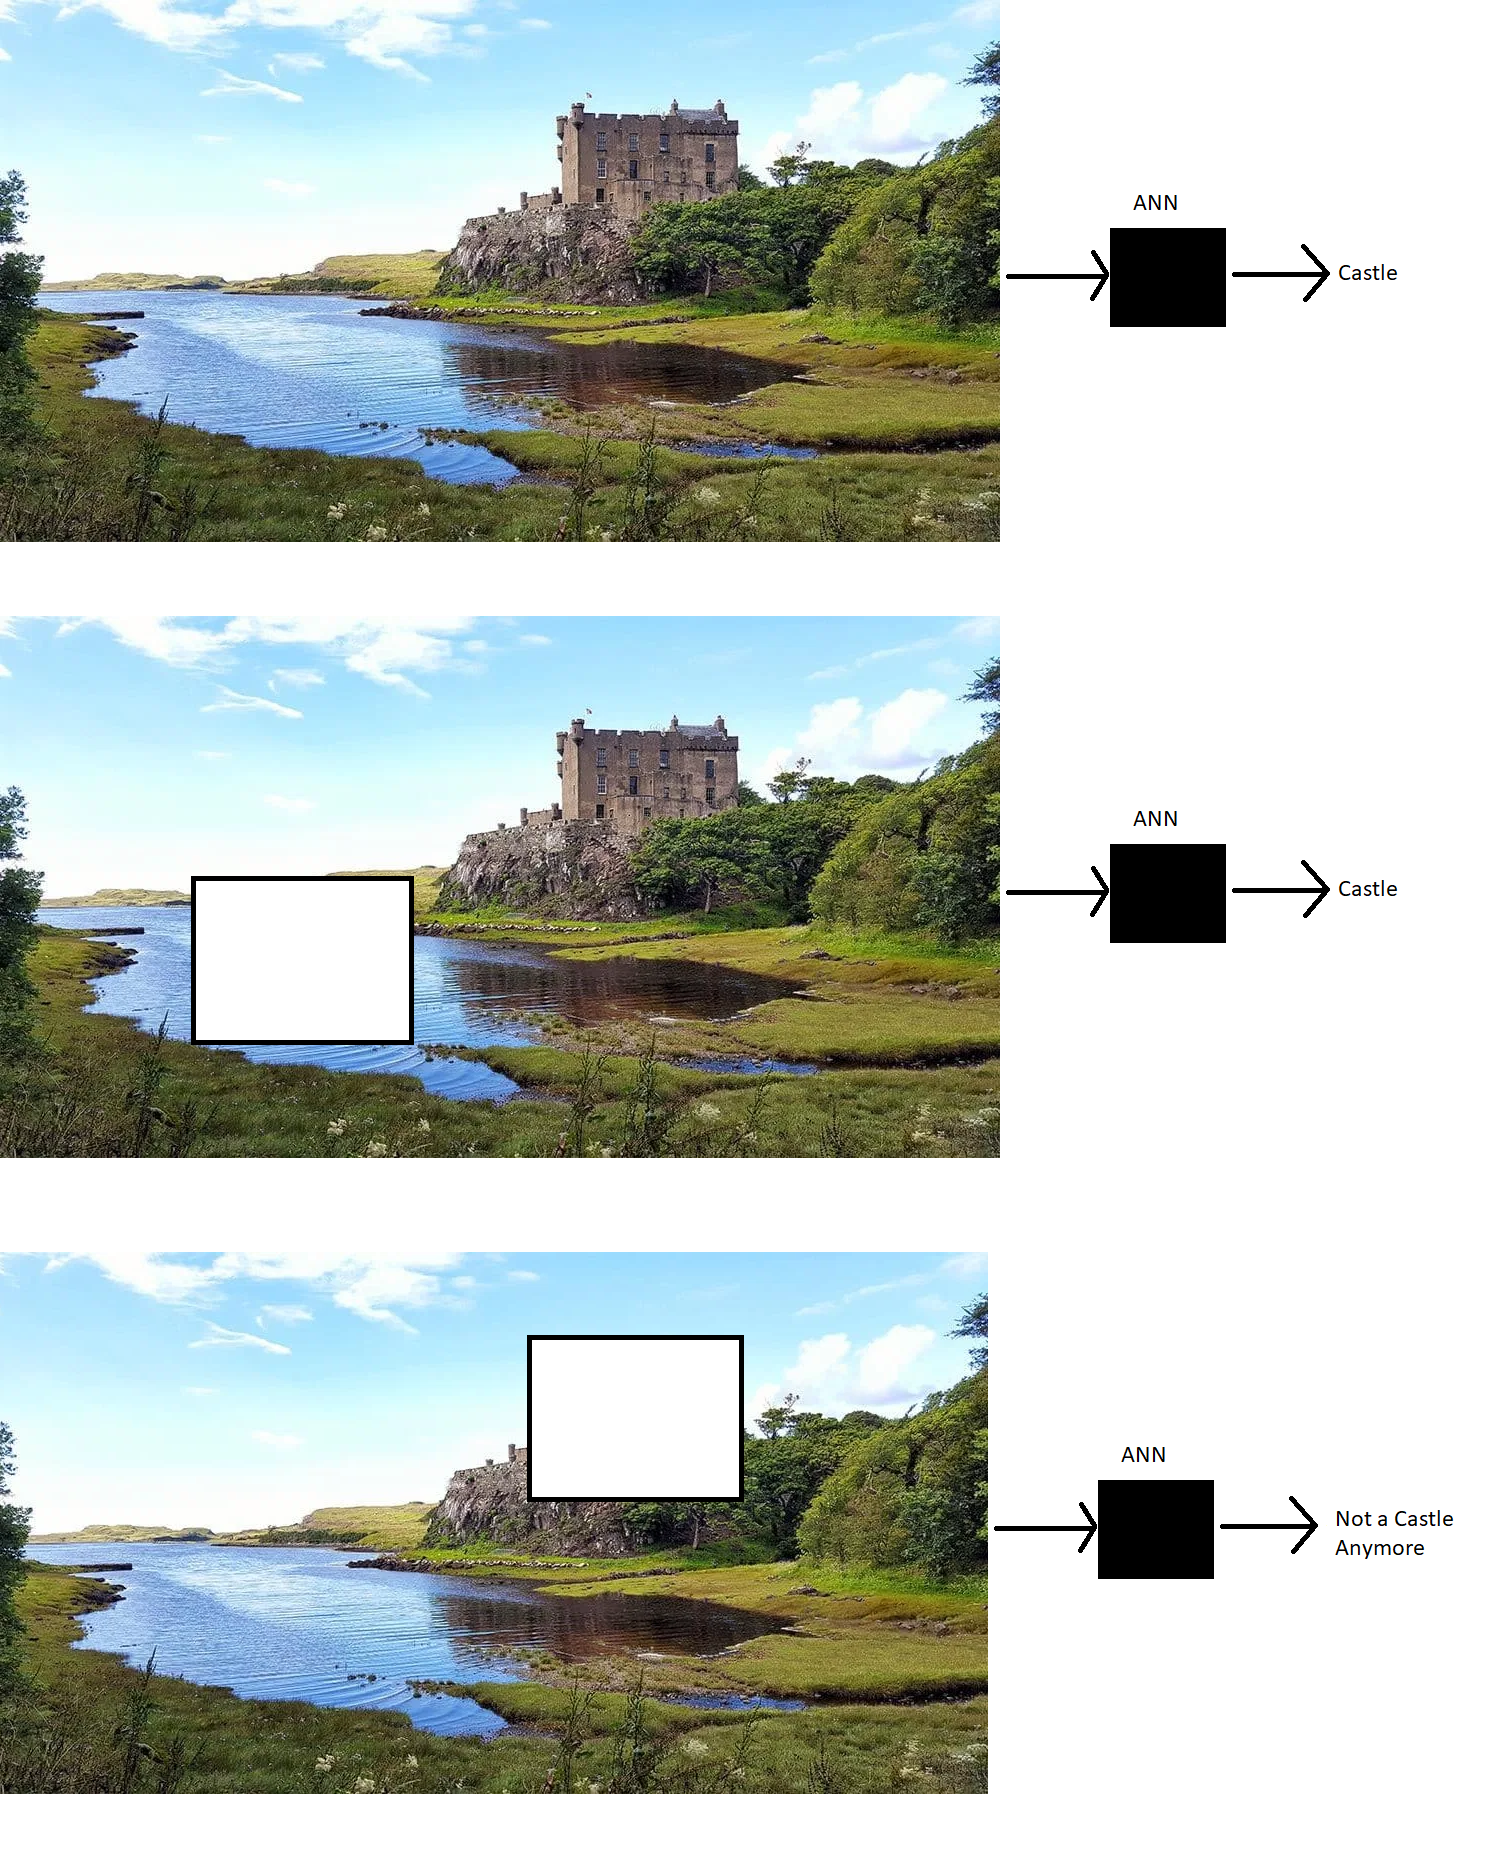
\includegraphics[width=\linewidth]{images/02_related_works/Garden-Dunvegan-Castle_Modified.png}
    \caption{Perturbation based approach visualized on an ANN trained to detect castles \cite{castle_image}}
    \label{fig:perturbation_approach}
\end{figure}

In the example above: \autoref{fig:perturbation_approach} the perturbation approach XAI tool would conclude that the pixels in the first rectangle are not important for the classification while the ones in the second one are. While seeming straight forward, this approach has two key disadvantages:

\begin{itemize}
    \item Assumes locality, \textit{meaning that it assumes that the output only depends upon the current input and the base rate of the model(the average output of the model).}
    \item Perturbations may introduce artefacts. \textit{In the above example you could imagine that a big grey rectangle is recognized if not as a castle, then at least as a concrete building. This is a particular issue when explaining text. The classifier might respond to grammatically incorrect sentences in a certain way which would be an unwanted side effect of said removal.}
\end{itemize}

\subsection{Function based approaches}

In this section we will cover the well-known Gradient x Input approach.

We will quickly reiterate some basics and then explain how this approach can be used to create an explanation. Let's say we have a classification function $f$ which takes a multidimensional input $x$. We now would like to know which direction/dimension was more important than the others. To find this dimension, we use following function: The \textit{Gradient}.

\begin{equation}
    \nabla f(x) = \frac{\delta f(x)}{\delta x}
\end{equation}

If we apply that \textit{Gradient} to $x$ like done above, we get a vector of partial derivatives of $f(x)$ for every dimension of $x$. We now know which direction has the largest impact on the classification. We can now look at that direction and determine from it which values of $x$ are the most responsible ones for the classification result. This can be done in the form of a \textit{Gradient x Input} matrix called an attribution map. For most applications, this works well but still has some issues. The gradient only tells us the importance of a dimension if we just take a tiny step which is very local information. Furthermore it suffers from \enquote{noise} (the explanation map does not form a clear structure but shows seemingly random information), an issue this thesis tries to address. This method serves as a solid conceptual basis for more involved explanation methods including the one we implemented \cite{GradientInput}.

\subsection{Surrogate-/ Sampling based approaches}

Sampling's main goal is speed. You quickly approximate a solution without guaranteeing that the solution is correct. This is a valid approach since computation power is still the biggest limiting factor concerning artificial neural networks. We will quickly look at one of these approaches: \textbf{local interpretable model-agnostic explanations (LIME)} \cite{Lime_paper}.


This method ignores the global underlying black box and only tries to provide an explanation for a single prediction. To achieve that goal, it generates a new dataset consisting of modified samples and runs them through the black box. Using this new dataset, lime then trains an interpretable model (we will come back to what an interpretable model is in \autoref{chap:basics}, for now just consider it a simple model which can be understood by just looking at its structure/code). Lime's model should be a good approximation of the original black box locally but does not have to be a good global approximation (see \autoref{fig:lime_global_local}). This kind of accuracy is called local fidelity \cite{Lime_shap_explained}. 


Throughout this thesis we will call the approximated model the \textit{explanation model} and the model we wish to explain the \textit{original model}.

\begin{figure}[H]
    \centering
    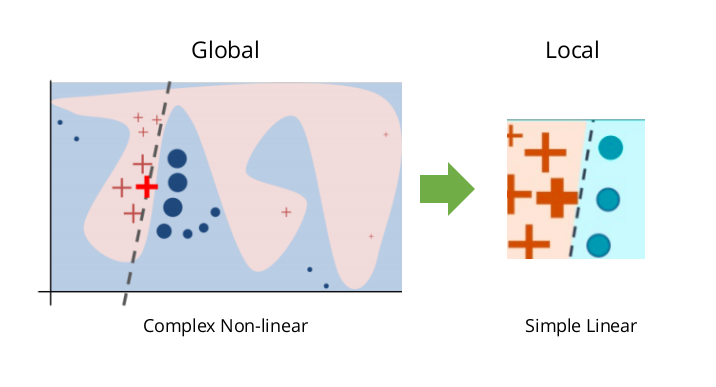
\includegraphics[width=\linewidth]{images/02_related_works/Lime_global_local.png}
    \caption{LIME localizes a problem and explains the model at that locality, rather than generating an explanation for the whole model \cite{Lime_paper}.}
    \label{fig:lime_global_local}
\end{figure}

The method we implemented, called shap, is actually a special implementation of Lime adding further rules to the algorithm making it more predictable but also less flexible. We will explain these differences in more detail in \autoref{chap:SHAP}.

\subsection{Structure based methods}

Structure based methods look at the structure of the ANN. We will briefly talk about the layer wise relevance propagation method. It tries to find subfunctions in the neural network. For example a part of the network which finds a certain pattern. We do this by starting from the output. Often, not always, we can detect a pattern, which part of the neural network is responsible to detect a certain output class. This can then be analyzed to realize what part of the input is responsible for a certain classification.\\

\begin{figure}[H]
  \centering
    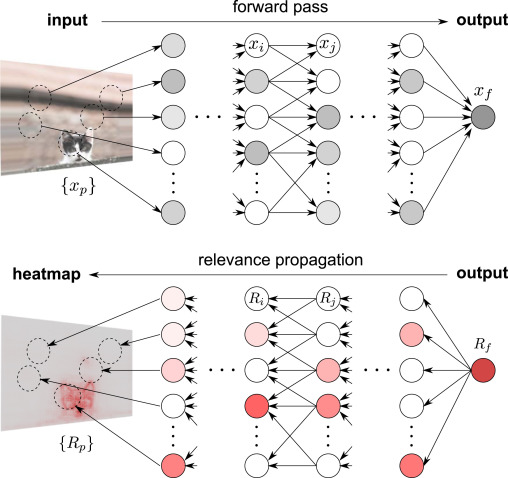
\includegraphics[width=\linewidth]{images/02_related_works/Layer wise relevance propagation2.png}
  \caption{Layer wise relevance propagation \cite{LRP}}
  \label{fig:layer_wise_relevance_prop}
\end{figure}

In \autoref{fig:layer_wise_relevance_prop} we see how the red inputs form the shape of a cat. We can then conclude, that the \enquote{activated} part of the ANN is a function detecting the shape of a cat.

This is a very powerful method with only one drawback, its implementation is very dependent on the shape of the neural network. Classifiers that do not use the traditional neural network shape cannot be analyzed using that method.

\subsection{Shap}

All of these approaches are valid, they each have their advantages and disadvantages. The method we will implement, shap, is actually a mixed approach picking tools from each basket to form a powerful explainer (\autoref{chap:SHAP}). Yet it suffers itself from a few disadvantages. We will go over in more details about those and how our work tries to address one of these issues (\autoref{ch:Results}).
%% LaTeX2e class for student theses
%% sections/content.tex
%% 
%% Karlsruhe Institute of Technology
%% Institute for Program Structures and Data Organization
%% Chair for Software Design and Quality (SDQ)
%%
%% Dr.-Ing. Erik Burger
%% burger@kit.edu
%%
%% Version 1.3.5, 2020-06-26

\chapter{Basic Concepts}
\label{chap:basics}

\textit{In this chapter we will go over some of the more fundamental concepts which are necessary to understand how explainers work in general and their challenges. Expert readers may skip this chapter.}

\section{Interpretability}

Interpretability is a rather vague concept which can be summarized in following statement: \enquote{can the average human understand it?}. This simple statement has multiple issues.
It is very unclear what that means in practice. A lot of work has been done to define that statement in the last few years \cite{lipton2017mythos}. The latter reference defines a few desiderata which models should have to be interpretable. We will go over some of them and explain what that means in our context of text classifiers.

\begin{itemize}
    \item \textbf{Simulatability}: In opposition to the opacity of artificial neural networks, simulatability is a property interpretable models need to have. The idea is, that a model is simulatable, if a person can contemplate the entire model at once in a \textit{reasonable} timeframe. This is important because it is possible to contemplate parts of artificial neural networks, and understand them because in itself they are very simple functions, but in such quantities, that it is impossible to contemplate them all at once. It also contradicts the idea that linear models are always interpretable. If complex enough, even a linear model is not humanly understandable.
    \item \textbf{Decomposability}: States that the model can be decomposed in parts which can be understood by themselves, without needing to understand the whole function. This notion of interpretability while being popular is controversial, because it excludes many models from being interpretable but I will make the argument that it is very much true. Humanly understandable means that one human can explain the model to another human. That is only possible if you can start somewhere, if you can put your explanation in logical following parts. This is how humans arguments, pick up information, a process called \textbf{active learning} \cite{activeLearning}. While a model might seem simple enough to be understood by the human mind, it needs to be decomposable so that a human can acquire the knowledge about the model in a structured way.
    \item \textbf{Algorithmic transparency}: While it is possible to understand how an algorithm works, it can be much more difficult to accept that the algorithm will provide the desired result. This is however an important part of Interpretability, if the algorithm cannot be trusted to work as intended, it is not really understood because the results are much more difficult to predict \cite{lipton2017mythos}.
\end{itemize}


Let's now analyze what that means in the case of text classification using artificial neural networks. It is obvious that we cannot provide any of the three desiderata for modern neural networks. It is thus necessary to take a detour to try to explain the model in an interpretable way. To do this we create another much simpler function, the explanation model, which approximates the result the original model provides. As mentioned in \autoref{ch:Introduction}, it cannot be guaranteed that this approximation is correct. While that should be criticized, it is the best we have. To achieve that goal we use three methods: \textit{Post-hoc analysis, local explanations} and \textit{explanations by example.}

\section{Post-hoc analysis}

Post-hoc analysis is a simple concept, consisting of statistical analysis specified after the data is seen. This makes the analysis method model agnostic, it can analyse any function, artificial neuronal networks among them. While there are (like discussed in \autoref{ch:stateOfTheArt}) methods which analyse the structure of the neural network to create an interpretable model, the post-hoc analysis does not care about the structure of the neural network. One major drawback with post-hoc analysis is that it is hard to discern between causality and correlation (\autoref{fig:postHocCausCorr}). This issue is also present with neural networks, since those are trained following the same Post-hoc analysis principle, and any correlation which isn't causality is very likely to also be present in the original model, hinting that the model cannot be used to provide proper classifications.

\begin{figure}[H]
    \centering
    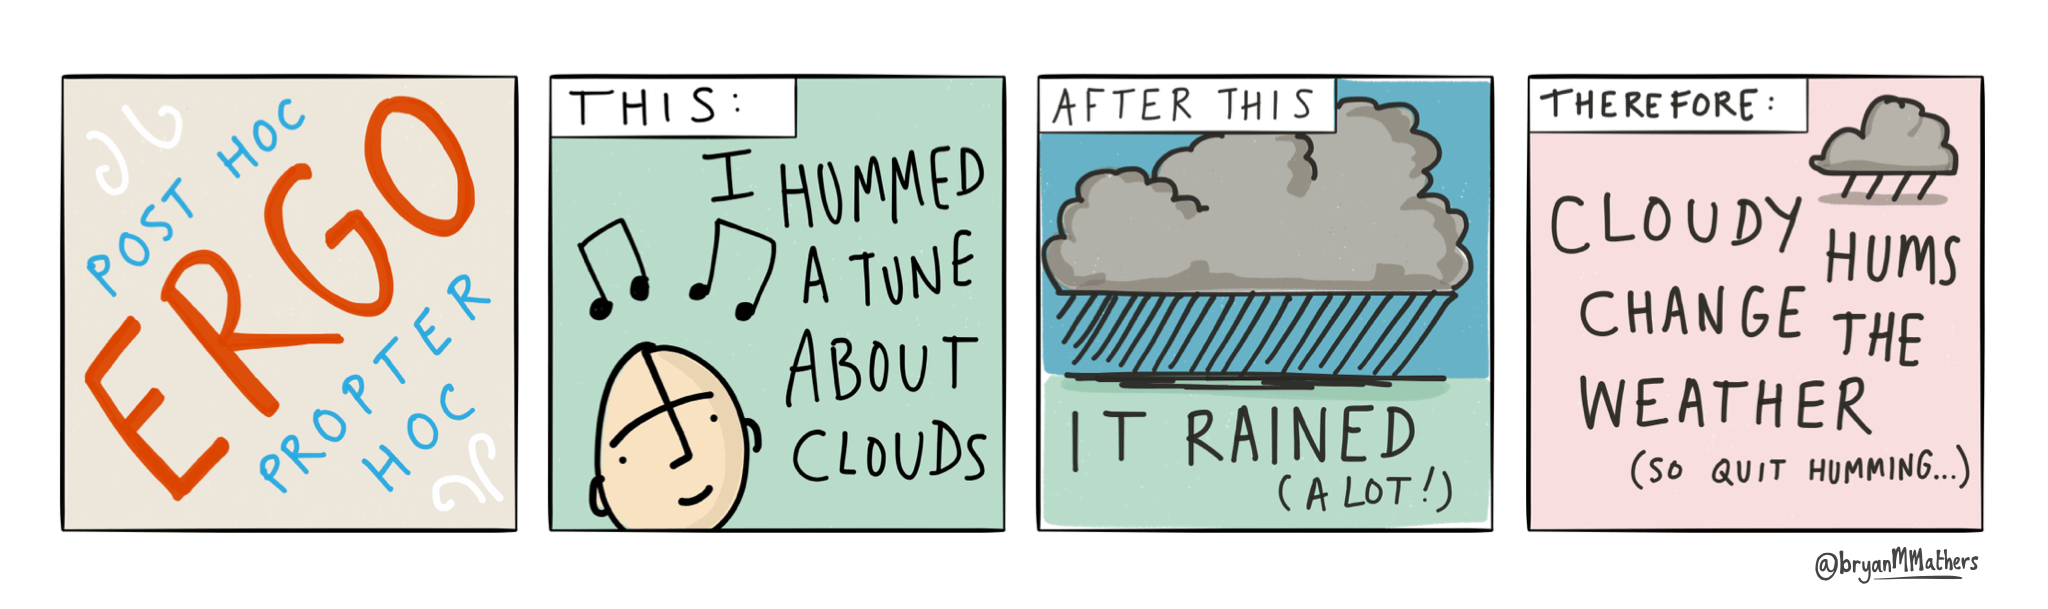
\includegraphics[width=\linewidth]{images/03_basics/Post-Hoc analysis.png}
    \caption{Post-Hoc causality vs correlation \cite{mathers_2017}.}
    \label{fig:postHocCausCorr}
\end{figure}


Again, what does this mean in our case of text analysis? Our inputs are the strings we wish to classify, the outputs are the classification scores. We can create an explanation model by altering the input and analysing its effects on the classification score. We have discussed one tool (lime) in \autoref{ch:stateOfTheArt} which works in this way and we will further look at how shap does it.

\section{Local Explanations \& Explanation by example}

The second method we are using is not trying to explain the entire original model, but only approximate it in a local context. This means, that our explanation model is only faithful to the original model for that one classification. This is necessary because the complexity of modern neural networks can greatly surpass anything which could be approximated with an interpretable function. This allows us to solve one of the big issues with neural networks, we can debug and notice possible mistakes. All three scenarios mentioned in \autoref{ch:Introduction} can now happen:

\begin{enumerate}
    \item Developers just need a hint on how to solve a problem and even an incomplete explanation of a neural network enables them to code it in a humanly understandable way.
    \item We understand a fraction of how the artificial intelligence makes a decision but it is enough to disqualify it. This is especially important if some unwanted behaviour like biased \textit{(racist/sexist/...)} decisions are revealed.
    \item We understand a fraction of how the artificial intelligence makes a decision and its approach feels plausible to humans.
\end{enumerate}

For text-classifiers, this means that we get an explanation as to why a specific text got its classification score. It proposes an explanation model which approximates the original model for this one text. It can and will substantially diverge from the actual model, but its results will be consistent for this one specific text. The hope is that this approximation picks the parts of the original model which are relevant for the classification of this one text, creates its own simpler model using them and ignores the rest of the original model \cite{ExampleBasedExplanation}.

\begin{figure}[H]
    \centering
    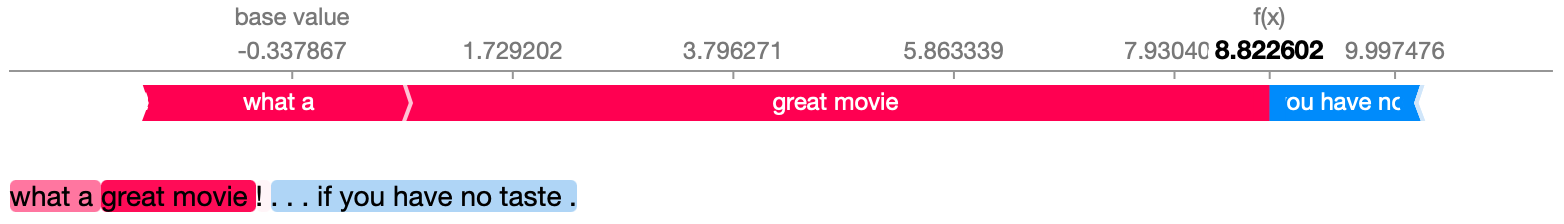
\includegraphics[width=\linewidth]{images/03_basics/sentiment_analysis_plot_movie.png}
    \caption{Linear approximation model \cite{shapDocs}}
    \label{fig:shapMovieExplained}
\end{figure}

Above we have an example of a linear explanation model, which provides the same result as the original model $f(x)$, but is much simpler to understand. The base value is the value you would get if you classified an empty text. The red text snippets are the words which move the classification score to a greater value, the blue ones to a lower value. At the end you get the same classification score as the classifier $f(x)$ produces.

\vspace{2cm}

The tool we implemented provides a post-hoc local explanation. We will now go into detail how it achieves that.
%% LaTeX2e class for student theses
%% sections/evaluation.tex
%% 
%% Karlsruhe Institute of Technology
%% Institute for Program Structures and Data Organization
%% Chair for Software Design and Quality (SDQ)
%%
%% Dr.-Ing. Erik Burger
%% burger@kit.edu
%%
%% Version 1.3.5, 2020-06-26

\chapter{Shapley additive explanations (shap)}
\label{chap:SHAP}

\begin{figure}[H]
    \centering
    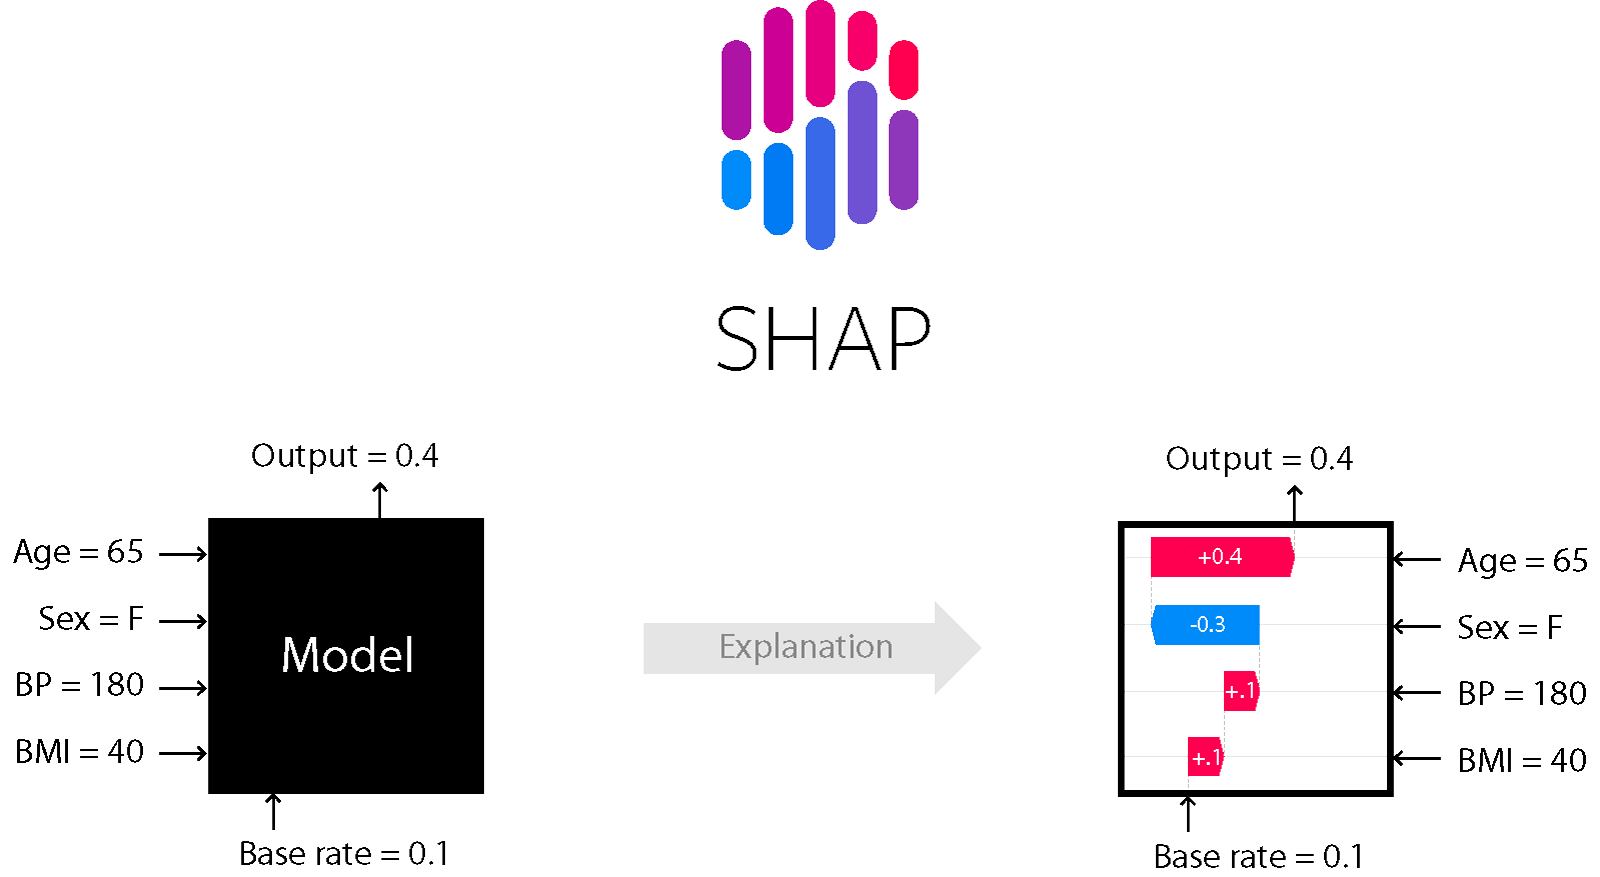
\includegraphics[width=\linewidth]{images/04_shap/ShapExplanationVisualized.png}
    \caption{Visualization of a shap explanation \cite{shapDocs}}
    \label{fig:shap_visualization}
\end{figure}


\section{General idea}

The human mind is astonishingly good at detecting patterns. It achieves this at an incredible rate still unmatched by our most powerful supercomputers \cite{patternRecognitionPsychology}. The issue is, that once a pattern is recognized, it gets rather hard to \enquote{forget} it even if it is a so called \enquote{false pattern}. This false pattern recognition is called apophenia and is considered a massive roadblock to creating an explanation model, because it severely limits the ability to understand the explanation model when presented to the user. If the user thinks he understood the explanation model and then gets another example explanation which contradicts his understanding of the explanation model, psychologically this is very confusing. 

\vspace{0.5cm}

A simple solution to this problem is to aid the human pattern recognition by defining rules that cannot be broken inside the approximation model. We will go over detail about these rules and why they make sense. This obviously doesn't eliminate the risk of apophenia but should decrease it significantly.

\vspace{1cm}

\textit{Please note that the psychological aspect was not explored in detail by the original shap paper. This is my own interpretation and argumentation as to why their work is a revolutionary approach to balance accuracy and interpretability in the context of neural network explanations. This is done because my work tries to improve the interpretability of the explanations by tackling above mentioned psychological barriers.}

\section{Competitive Game Theory}
\label{section:compGameTheory}

Game theory is a simple concept, where you study mathematical models of the interplay between rational decision makers. The most known example is the prisoners dilemma shown in \autoref{fig:prisonersDilemma}. 

\begin{figure}[H]
    \centering
    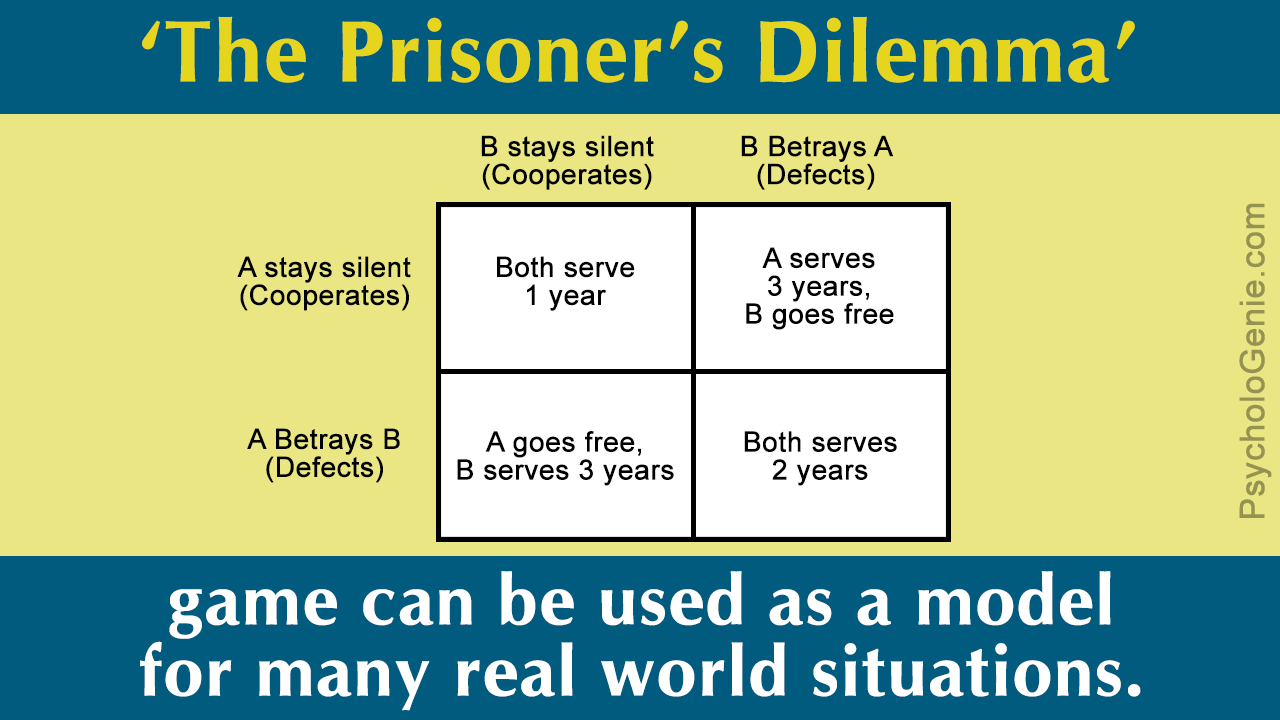
\includegraphics[width=\linewidth]{images/04_shap/Prisoners dilemma.png}
    \caption{Prisoners Dilemma \cite{psychologenie_2014}}
    \label{fig:prisonersDilemma}
\end{figure}

Game theory looks at how everyone should behave individually for the best outcome, and how a group of people should behave for the best outcome. The differences can then be discussed and often yield interesting properties. Competitive game theory is a subcategory of game theory, where a positive outcome for one \enquote{player} yields a negative outcome for another.

In our text classifications, this concept is used to determine the influence text-snippets have on the classification. Shap looks at the \textit{individual} influence of a single word, and then at how its context influences its meaning. For example the following text: "Jesus word is the word of God" will most likely be classified as being nearly 100\% christian, \textit{instead of being atheist}. If we remove the word Jesus from the text, it becomes as follows: "word is the word of God" which will also most likely be classified as nearly 100\% christian. Therefore individually, the word \textit{Jesus} does not influence the classification, but we intuitively know that it very much does or at least should. To find a more accurate value, to take the context into account, Shap removes multiple words in different orders and then combines the classification score differences using competitive game theory to find a more accurate value for that text-snippet.

\section{Shapley Properties}
\label{section:shapleyProp}

The values which determine the influence of each element introduced into the original model are called \textbf{shapley values}. They satisfy three very important properties meant to improve the interpretability of the results:

\begin{itemize}
    \item \textbf{Local Accuracy: } For the original input, the approximation model exactly matches the output of the original model.
    \item \textbf{Missingness: } This property is very misleading and should not be considered important. As described in the original shap paper \cite{shapPaper}: If the missing of a feature in  the original model does not change the result of the original model, then it should not have any impact in the approximation model either. This seems to contradict the use of competitive game theory and it does. I will directly quote the author of the shap paper Scott M. Lundberg when asked about this: \vspace{0.5cm}\newline
    \textit{\enquote{The missingness property is really just a minor book-keeping property to close a loop hole. It is required since local accuracy is specified as a linear model and x' [The input of the approximated model] could in theory have some zero entries (meaning the input is already missing [in the original input]). These zero entries mean that local accuracy would still hold no matter what phi values correspond to those entries, so to have a unique solution we need to constrain them to be 0 (which is what we want since they are missing already and so have no impact). In practice for SHAP we will never consider a feature to already be perfectly missing unless that feature's value is constant over the whole background dataset \cite{slundbergMissingness}.}} \newline
    \vspace{0.5cm} \newline
    To sum it up, it means that if a feature, meaning an indivisible input, is not present in the original input, it shouldn't play any role in the explanation.
    \vspace{0.5cm} \newline
    \item \textbf{Consistency:} if the importance of a feature increases because the original model has changed, then its importance should not decrease in the explanation model. This property makes the results much more interpretable, because consistency is an important part of interpretability.
\end{itemize}

\section{Examples for explanations of text based classifiers}

\begin{figure}[H]
    \centering
    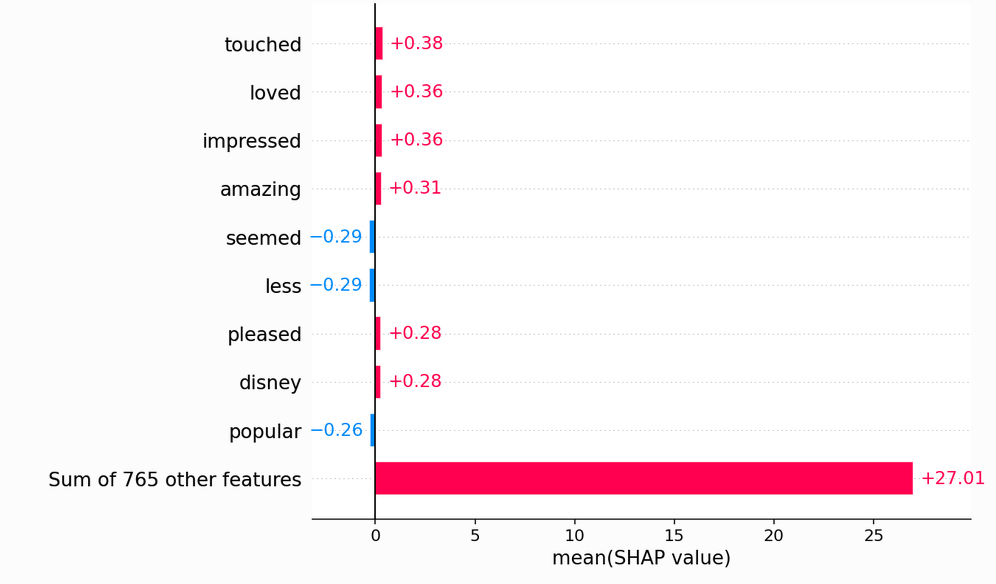
\includegraphics[width=\linewidth]{images/04_shap/ShapExplanationExample1.PNG}
    \caption{Shap explanation example \cite{shapDocs}}
    \label{fig:ShapExplEx1}
\end{figure}

In \autoref{fig:ShapExplEx1} we see the top 9 features which have the largest influence on the classification with their respective shapley values. These values are getting dwarfed by the sum of all other features, but it helps to give an idea about how the classifier works. If the top features should not be part of the classification process, we can suspect that something is wrong with the classification.


This can be rather difficult, especially, if words which only show their importance in their respective context are part of the top 10 most important features. This issue is one we are going to try to approach in \autoref{ch:Results} and suggest how to improve the interpretability of the explanation by using different text hierarchies.

% Example of where interpretability does not work

\subsection{Example where the explanation is difficult to understand because the context is missing.}
\label{section:ExplanationExample}

The following email has been classified as being 99\% christian:

\noindent\rule[0.5ex]{\linewidth}{1pt}
From: jenk@microsoft.com (Jen Kilmer)\\
    Subject: Re: Homosexuality issues in Christianity\\
    Organization: Microsoft Corporation\\
    Lines: 27\\
    
    In article <May.11.02.36.59.1993.28108@athos.rutgers.edu>\\ dps@nasa.kodak.com writes:\\
    >In article 15441@geneva.rutgers.edu, loisc@microsoft.com (Lois\\ Christiansen) writes:\\
    
    >|>he can, especially homosexuality.  Let's reach the homosexuals for\\ Christ.\\
    >|>Let's not try to change them, just need to bring them to Christ.  If He\\
    >|>doesn't want them to be gay, He can change that.  [....]\\
    
    >don't hate the people.  I don't.  I don't hate my kids when they do\\
    >wrong either.  But I tell them what is right, and if they lie or don't\\
    >admit they are wrong, or just don't make an effort to improve or\\
    >repent, they get punished.  I think this is quite appropriate.\\
    
    Note the difference here. One is saying, if *Christ* disagrees with\\
    a Christian being gay, *Christ* can change that.\\
    
    The other is saying, if *I* think being gay is wrong, that a Christian\\
    cannot be gay, *I* need to tell them to change.\\
    
    
    As Lois said, and as before her Paul wrote to the believers in Rome,\\
    WHO ARE YOU TO JUDGE ANOTHER'S SERVANT?\\
    
    -jen\\
    
    --
\cite{Newsgroups20}\\
\noindent\rule[0.5ex]{\linewidth}{1pt}

The classification is obviously correct, we will now run shap trying to find out why that classification score was reached:
\begin{table}[H]
    \centering
        \begin{tabular}{c|c}
                Feature name & Feature importance \\ \hline
                rutgers & 0.040224 \\
                athos & 0.036232 \\
                geneva & 0.030274 \\
                1993 & 0.025009 \\
                christ & 0.022898 \\
                article & 0.021479 \\
                writes & 0.019735 \\
                com & 0.019473 \\
                paul & 0.016807 \\
                don't & 0.014403 \\
                nntp-posting-host & 0.010084 \\
                nntp-posting-host & 0.010084 \\
                atheism & 0.008166 \\
                christian & 0.00862 \\
                christianity & 0.008166 \\
                christians & 0.00797
            \end{tabular}
            \caption{Example where it is difficult to interpret what the classifier does.}
            \label{tab:example_bad_interpretation}
\end{table}

Here we find out, that the classification is being done by looking at the header, the email provider. If studied in more detail, it would become clear, that the training dataset is flawed, all christian emails come from the same email provider. The classifier is not doing what it should, it reaches the correct classification, but if the header is missing, the classification result would become mostly random. Coming to this conclusion takes a lot of work though, because if we didn't provide the original text, you would be confused about the presence of words like \enquote{rutgers}, \enquote{athos} or \enquote{don't}. These are so dependent on their context, that by themselves they do not provide any information at all. This problem is particularly apparent for text-classifiers and are the reason we chose them. In \autoref{ch:Results} we will suggest a method to remedy that particular issue.

\vspace{1cm}

We will now present the framework which was developed to  help analyse multiple explainers.
\chapter{Framework evaluation}

In this chapter we will look at an evaluation framework developed at the institute for program structures and data organization. We will go over its goal, a basic overview of its components and how it is meant to be used. Finally we will talk about the challenges of implementing an analysis using shap withing this framework.

\section{Goal of the framework}

As discussed in \autoref{ch:Introduction}, tools are essential for the mass adoption of new technologies. XAI is still met with a lot of scepticism and rightfully so, every new technology should be tested extensively before it is widely adopted. Our evaluations took over a year to produce and we believe that by using the same framework we developed other scientists can create further evaluations in much less time.

\section{Overview of the framework}

\textit{The following description of our framework is a simplification, please refer to the documentation or actual code for a truthful representation. This is especially true for the overview diagram \autoref{fig:framework_overview}. This was done for overview purposes.}


The framework can be divided into 5 distinct parts which in theory should be exchangeable without having to modify any of the other 4 parts.

\begin{enumerate}
    \item Resources, \textit{data set, embedding, preprocessing}
    \item Classifiers, \textit{abstract classifier class, fit function, classification function}
    \item Explainers, \textit{abstract explainer class, explain function}
    \item Analyses
    \item Output, \textit{functions to save the analysis data in csv files for further processing.}
\end{enumerate}

In \autoref{fig:framework_overview} I provide the overview over the five components and their interfaces.

\begin{figure}[H]
    \centering
    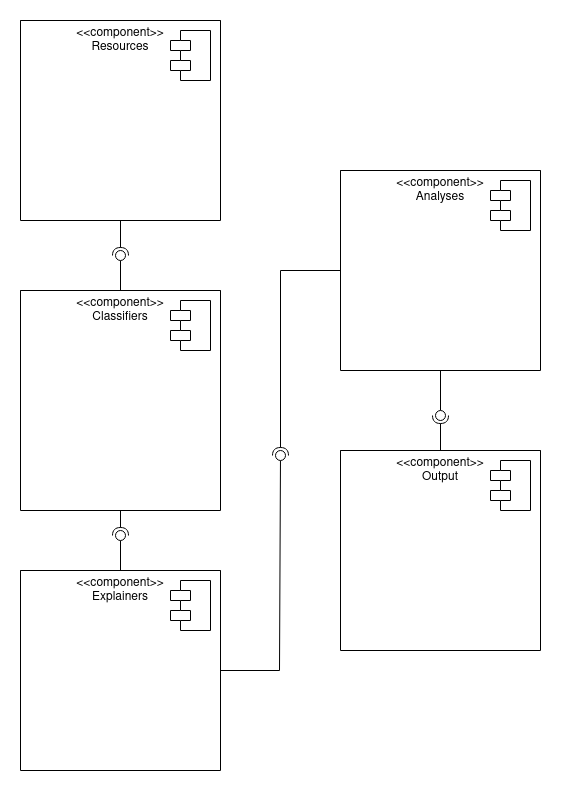
\includegraphics[width=\linewidth]{images/05_framework_eval/Component_diagram_overview_framework.png}
    \caption{Component diagram, framework overview}
    \label{fig:framework_overview}
\end{figure}

\subsection{Component 1: Resources}

\begin{figure}[H]
    \centering
    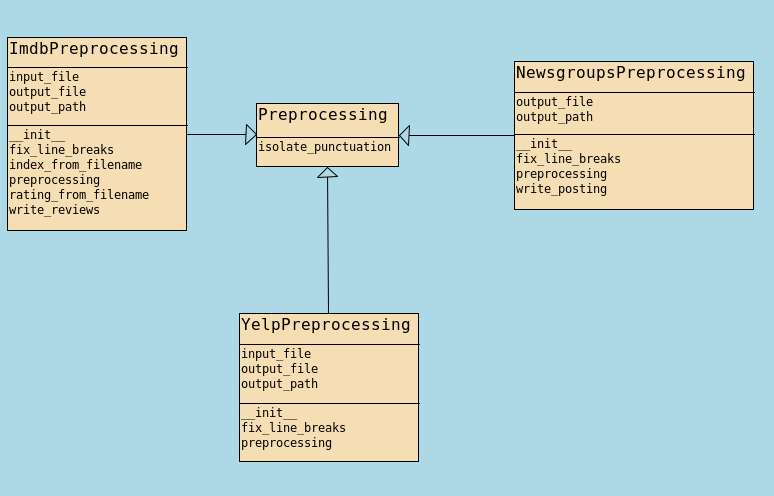
\includegraphics[width=\linewidth]{images/05_framework_eval/Preprocessing.png}
    \caption{Preprocessing}
    \label{fig:preprocessing}
\end{figure}

The \textit{Resource} component includes the data set and any preprocessing functions which might be needed to prepare/modify the given dataset. If you decide to use/include your own dataset, and you need to preprocess your data, you should make a child class to the preprocessing class.

\subsection{Component 2: Classifiers}

\begin{figure}[H]
    \centering
    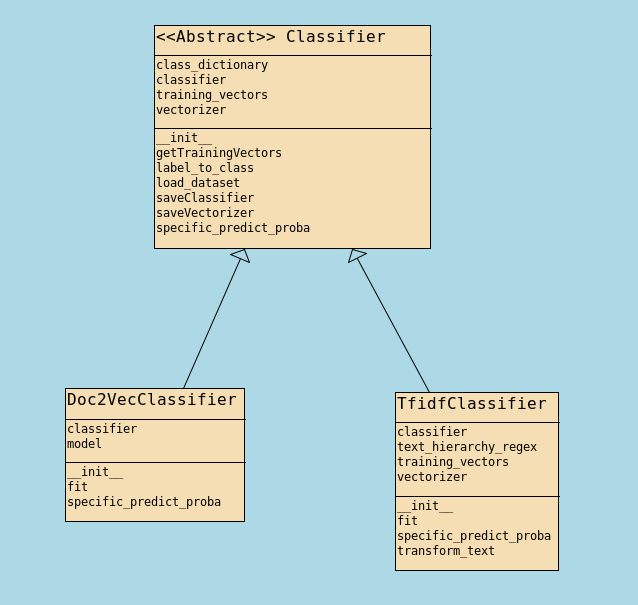
\includegraphics[width=\linewidth]{images/05_framework_eval/Classifiers.png}
    \caption{Classifiers}
    \label{fig:Classifiers}
\end{figure}

The \textit{Classification} component includes the classifiers, with functions to train or load them. Pretrained classifiers are not supported yet, but you can save a classifier after training it. A new classifier should be a child to the abstract classifier class.

\subsection{Component 3: Explainers}

\begin{figure}[H]
    \centering
    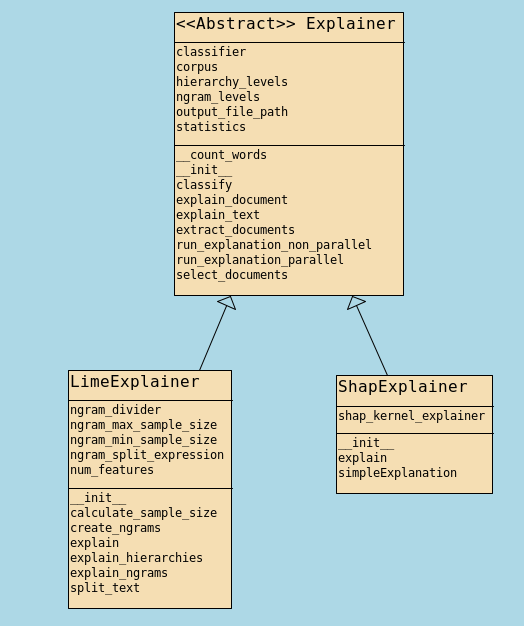
\includegraphics[width=\linewidth]{images/05_framework_eval/Explainers.png}
    \caption{Explainers}
    \label{fig:Explainers}
\end{figure}

The \textit{Explainer} component includes the explainers and functions to explain texts or documents.
If you wish to add another explainer, it should be a child class of the abstract explainer class. This can be challenging, because the output format of the explanation must follow a certain format.

\subsection{Component 4: Analyses}


\begin{figure}[H]
    \centering
    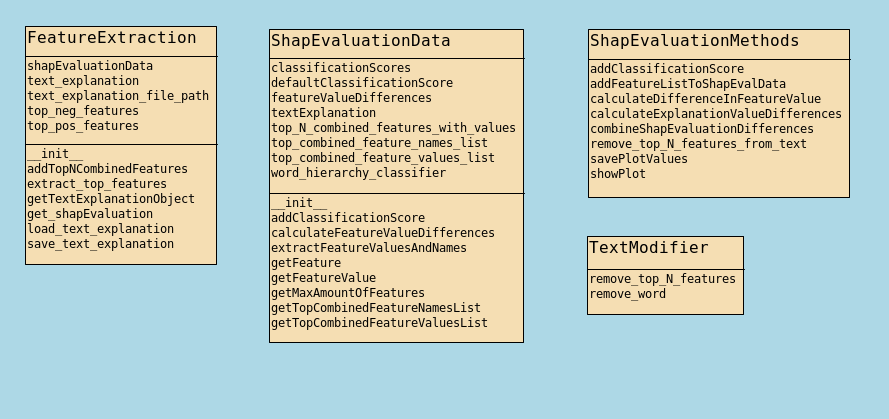
\includegraphics[width=\linewidth]{images/05_framework_eval/Analyses.png}
    \caption{Analyses}
    \label{fig:Analyses}
\end{figure}

The \textit{Analyses} component is much more loosely structured. The user should be able to freely carry out his own analyses.

\subsection{Component 5: Output}

\begin{figure}[H]
    \centering
    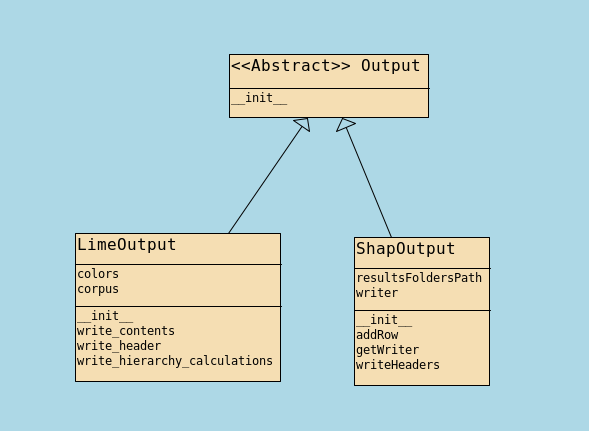
\includegraphics[width=\linewidth]{images/05_framework_eval/Output.png}
    \caption{Output}
    \label{fig:Output}
\end{figure}

The \textit{Output} component defines how the analysis data is saved. Here we break the modularity of the framework. If you add another analysis, it is very likely, that you will have to write your own output child class. We are working on improving this, hopefully this will not be necessary in the future.

\section{Intended use}

We do not expect you to be satisfied with the provided components, depending on the scope of your work, you might want to exchange multiple components. Nonetheless, you might still find our framework useful. A major difficulty in setting up an XAI analysis, is that it can take months of coding to get an analysis to work properly. We suggest you build it step by step, working on one component at a time and using our provided ones to check for mistakes and provide structure to your workflow.

\section{Shap Implementation using our framework}

There are many different implementations of the shap algorithm, notably \textit{gradientexplainer, deepexplainer, linearexplainer} and \textit{kernelexplainer}. Except for \textit{kernelexplainer}, each one is specialized for a special type of neural network. Since our framework is intended to have modular, interchangeable components, I tried to use \textit{kernelexplainer} in our analysis.

During development, I encountered following challenges:
\begin{itemize}
    \item Kernelshap's poor performance
    \item Kernelshap's resource requirements
    \item Missing required function in the library
\end{itemize}

Let's go over them in detail:
\subsection{Poor performance}

Kernelshap is model agnostic (meaning it can work with every type of artificial neural network) which meant that it could not be optimized according to the shape of the respective neural network. Because of that, generating an explanation for a single text took between 5 to 10 minutes on my workstation and the institutes server alike. This is very hindersome during development. While impossible to completely solve, I took some measures to cache as many steps as possible.

\begin{lstlisting}
    def saveClassifier(self, classifier_out_file):
        print("saving classifier: ", classifier_out_file)
        dump(self.classifier, classifier_out_file)

    def saveVectorizer(self, vectorizer_out_file):
        print("saving vectorizer:", vectorizer_out_file)
        dump(self.vectorizer, vectorizer_out_file)
\end{lstlisting}

\subsection{Resource requirements}

Kernelshap uses a lot of memory. You need around 10 GB of ram to run an explanation for a single text. Since this is hard-coded into the shap library, not many optimizations were possible. I upgraded my hardware and added parameters to limit the amount of texts being explained in parallel.

\begin{lstlisting}
    if RUNNING_ON_SERVER:
        # how many cpus are used during parallelization. With more than 2 my pc crashes
        AMOUNT_OF_CPU_CORES = 10
    else
        # how many cpus are used during parallelization. With more than 2 my pc crashes
        AMOUNT_OF_CPU_CORES = 2
\end{lstlisting}

\begin{lstlisting}
    pool = mp.Pool(shap_constants.AMOUNT_OF_CPU_CORES)
    # the actual explanation is now saved inside of this array of textExplanations
    text_explanations = pool.starmap(self.explain_document, explain_documents_arguments_iterable_tuple)

    pool.close()
\end{lstlisting}

\subsection{Missing functions in library}

Shap is a young explainer in active development. A few API functions which were necessary for my analysis weren't provided, so I had to write them myself. One example is that it was not possible to get a list of the top N features which have the most impact on the classification score. It was especially challenging to write this function, since the documentation on how to extract these values is nonexistent. It was thus necessary, to analyse the library's code line by line.

\begin{lstlisting}
def get_top_features_of_specific_class(index: int, amount_of_features: int, shap_values, feature_names, pos_or_neg_val: str):
    '''
    :param index: 0 for first class, 1 for second class, doesn't matter since the pos ones for one class are the neg
    ones for the other but we encourage to only use class 1 to avoid confusion.
    :param amount_of_features: how many features should be presented in the explanation
    :param shap_values: I believe those to be of the same format as the model output: in our case the model outputs
    2 values so the shap_values are a list with two arrays. first array: shapley_values[0] holds the features which are
    believed to nudge the explanation towards class 0,     shapley_values[1] hold the values which are believed to
    nudge the explanation towards class 1.
    :param feature_names: the model takes text transformed in vector form, the explanation should output text again.
    feature names map the vector values back to text.
    :return: top <amount_of_features> for class <class_number> as a table.
    '''
    # extract top features either positive or negative
    if pos_or_neg_val == "pos":
        shap_class_values = shap_values[index].mean(axis=0)
    elif pos_or_neg_val == "neg":
        shap_class_values = - shap_values[index].mean(axis=0)
    elif pos_or_neg_val == "combined":
        shap_class_values = np.abs(shap_values[index]).mean(axis=0)

    importance_df = pd.DataFrame([feature_names, shap_class_values.tolist()]).T
    importance_df.columns = ['feature-name', 'shap_importance']
    importance_df = importance_df.sort_values('shap_importance', ascending=False)
    return importance_df.head(amount_of_features)
\end{lstlisting}

%\subsection{Adapting for text-input}

\section{Framework outlook}

The Framework is still a work in progress. Most notably it lacks documentation and overview to reduce the entry barrier. That being said, once its architecture adheres to \autoref{fig:framework_overview} and some basic documentation is provided, I believe that it has the potential to contribute in a significant way to future XAI analyses.
\chapter{Results}
\label{ch:Results}

\section{Challenges evaluating XAI Explanations}

As we've seen in the previous chapter, shap is a very specific recently proposed method to generate an explanation. Its algorithm follows rules and gives a result which exactly matches the output from the classifier \cite{NIPS2017_7062}.

\begin{quote}{Scott M. Lundberg, Su-In Lee \cite{shapPaper}}
    When approximating the original model $f$ for a specific input $x$, local accuracy requires the explanation model to at least match the output of f for the [\textit{original input $x$}]
\end{quote}

Even if, using \textit{kernelexplainer}, the result is approximated, this approximation error is not directly accessible, because competitive game theory produces a feature value which when all feature values are summed up, exactly matches the classification result \cite{shapPaper, compGameTheory}. Nonetheless there are multiple possibilities to evaluate the quality of an explanation.

\section{Dimensions of the explanation quality}

I propose to categorize explanation qualities into three categories: \textbf{Accuracy, Interpretability} and \textbf{Resource-requirements.} These are not independent, we expect accuracy to increase with more allocated computational resource and vice-versa. Interpretability, \textit{meaning the ease with which the result can be understood} is expected to be negatively correlated with the accuracy. The more features that are analyzed and presented to the data analyst, the more difficult it gets to interpret the explanation.

It is important to keep those interactions in mind when tweaking parameters of the explanations. A definitive advice on how to set those parameters will not be possible because it is unclear how important each dimension is for the user.

In this thesis we will not be able to tackle all of these dimensions and will focus on the accuracy and interpretability ones.

\section{Necessary characteristics to analyse XAI results}

The principle is simple, we've seen above that to evaluate an explanation we need to compare it to another explanation to get useful results. Following properties need to be fulfilled for an evaluation method to be of worth:

\begin{enumerate}
    \item Be able to generate a theoretically unlimited amount of explanations for each parameter tweak.
    \item Be able to pinpoint the influence of a single parameter (or a clear defined combination of multiple parameters).
    \item Be able to theorize about the results on a \textbf{global} level (See \autoref{fig:ShapExplEx1}), \textit{meaning that the influence of tweaking one or multiple parameters can be logically understood or at least theorized about by looking at a multitude of explanations}. \textit{If the tweaking of a parameter results in chaotic changes which are not understood, tweaking that parameter is pointless}.
    \item \textit{(optional but desirable)} Be able to theorize about the results on a \textbf{local} level, \textit{by looking at a tuple of explanations of a single corpus with different parameters.}
\end{enumerate}

While the first three points are rather obvious, the last one might be a bit controversial and I will try to explain my reasoning. The goal of text-explanations is mostly to debug classifiers, to understand where they are failing and to fix issues in the underlying data. Examples like biased data, inadvertently pre-classified data (see \autoref{section:ExplanationExample}) come to mind. These issues are not always visible on a global scale. A lot of times the classifier uses shortcuts like detecting email-providers only on certain data entries which will not be visible when looking at a multitude of explanations. Some issues will not be detectable on a global approach, so explanations should not only focus on the entirety of the data-set. Since this is the expected use case for someone implementing/using shap, tweaking parameters of his implementation to learn more about a classification issue in a single classification is an important use case and it would be desirable that tweaking a parameter has an immediate effect on this single classification. This will be discussed in more detail in \autoref{ch:outlook}.


\section{Parameter: Text hierarchy}

One important parameter we will evaluate is the text-hierarchy, defining which entries shap considers atomic entities \textit{(which cannot be divided)}. This is important, because the user can only process a limited amount of information at once \cite{Baecker2014}, but the length of that information plays a secondary role, as long as each chunk of information is perceived as one \cite{Fountain2012}.

\subsection{Dataset}

The dataset used to generate these results, is a collection of christian/atheism themed emails provided by the Newsgroups20 \cite{Newsgroups20} dataset. It is composed of 717 emails. We fitted a binary tfidf classifier for each text hierarchy supposedly classifying the emails in atheist and christian categories. Using the 80/20 rule (80\% training data, 20\% test data) our classifiers never dipped below 90\% accuracy on any of our analyses (they are refitted on each run). The dataset and our approach is not ideal though, and can rightfully be criticized which we try to do in \autoref{sec:critique}.

\subsection{Context importance by text hierarchy}


\begin{table}[H]
    \centering
    \begin{tabular}{c|c}
         \textbf{Text-Hierarchy} & \textbf{Regex}\\ \hline
         Word & \verb/\b[\w|'|-]+\b/ \\
         Sentence & \verb/[^(.|?|!|\n)]+/ \\
         Paragraph & \verb/((?:[^\n][\n]?)+)/ \\
         2-gram & \verb/\b[\w|'|-]+\b\W+\b[\w|'|-]+\b/ \\
         ... & ...
    \end{tabular}
    \caption{Text Hierarchies}
    \label{tab:textHierarchies}
\end{table}

We will now try to evaluate the explanation results by evaluating the Newsgroup20 \cite{Newsgroups20} dataset with different text-hierarchies. For that purpose we used following formula:

\noindent\rule[0.5ex]{\linewidth}{1pt}

\textbf{\begin{multline}
\label{contextEvalFormula}
\mathrm{contextInfluence}(w’) = \\
| (\mathrm{classificationScore}(W)- \mathrm{classificationScore}(W\backslash w')) - \mathrm{shapFeatureImportance}(w') |
\end{multline}}

\textit{$w'$: The feature which had the most impact in the classification according to shap} \\
\textit{$contextInfluence(w')$: The importance of the context of the word w' according to shap} \\
\textit{$classificationScore(W)$: The classification score the classifier gives the text W}\\
\textit{$classificationScore(W \backslash w')$: The value the classifier gives the text W without the word w'}\\
\textit{$shapFeatureImportance(w')$: The feature importance shap gives the word w'}

\noindent\rule[0.5ex]{\linewidth}{1pt}
\vspace{1cm}

In \autoref{contextEvalFormula} we compare the change of the classification score when we remove the feature w' with the feature importance shap gives w'. We averaged the context influence over the entire corpus. We repeated this but instead of only remove a single feature we removed multiple features (in descending feature importance order) at once and plotted these results in \autoref{fig:shapEvalResults}.


\begin{figure}[H]
\centering
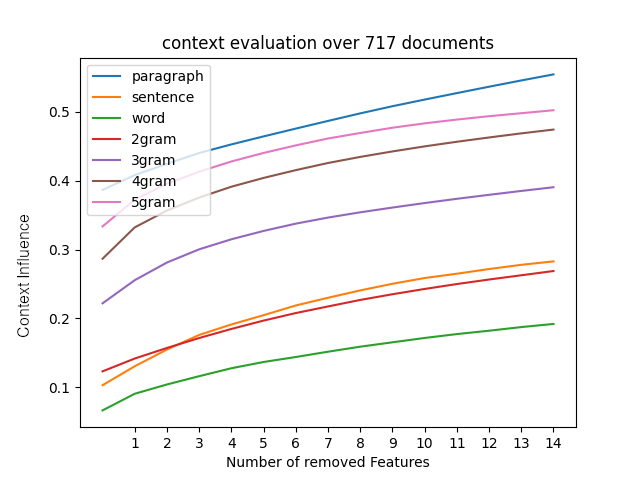
\includegraphics[width=\linewidth]{images/06_results/clemensEvalPlotAllSelectedDocsCombinedYAXIS.png}
\caption{Shap Evaluation Results.}
\label{fig:shapEvalResults}
\end{figure}

Now let's analyze what we did here. Calculating the importance of a feature by re-classifying the text without said feature is a simple perturbation based approach used before frameworks like \textit{lime} and \textit{shap} were developed. It does not take in account the context of a feature, an issue most recent approaches try to fix. The shap algorithm uses that method as well but adds more steps to it with the goal to \textbf{include the importance of the context} (\autoref{section:compGameTheory}), and to a smaller degree, make the explanation more intuitive (\autoref{section:shapleyProp}). So what \textbf{we are evaluating is how much weight the context of features has depending on the text hierarchy.}
\vspace{1cm}

With that information, let's analyze the produced plot:
\begin{itemize}
    \item As expected, generally, the bigger the group of text taken out of the original email, the more dependent it is of its respective context. This is what we would expect because each word can interact with other words in the text.
    \item This rule is however broken for sentences. A sentence has 14 words on average. Since we are working with emails, a sentence might be shorter. Nonetheless we would expect the contect influence to hover above the 5gram curve.
    \item The same could be said about paragraphs, meaning they hold multiple sentences and are just slightly more dependent on the context than 5grams. I would be careful though, the original dataset being emails, did not provide very structured paragraphs. Furthermore, I consider emails to be too short to draw any decisive conclusion about paragraphs based on our results.
\end{itemize}



The fact that sentences are less dependent on their context than any other random n-gram makes sense, they are, from a grammatical standpoint, a self contained part of the text. On average, it is much less dependent on its context than a string of words of the same length cutting in half two sentences (as shown in our analysis). Even though our findings are unspectacular, they allow us to substantially improve the quality of XAI text explainers. The goal of an explainer is to provide as much information as possible without overwhelming the user. \textbf{We can, instead of providing words to the user, provide entire sentences}, which massively increases the quality of the explanation (because of the reduced context importance) without overwhelming him with to much information. As a reminder, chunking allows the human brain to process sentences with n words much faster than n independent words \cite{ChunkingWikipedia}.

This is especially useful, if the previous explanation was not useful because the words provided were too dependent on their context (like shown in \autoref{section:ExplanationExample}). Our data shows that the per word influence of the context is reduced by 89,33 percent when comparing the context influence of sentences to the context influence of words.

\subsection{Critical analysis}
\label{sec:critique}

As mentioned before, there are a few points which could be improved in our approach, I will list them below:

\begin{enumerate}
    \item The emails are to short to analyse paragraphs properly. \textit{This is absolutely correct, in our analysis, we remove up to 15 features, and none of the emails in the dataset include over 15 paragraphs. The paragraph plot should not be used to make any conclusion and we only formulated a suggestion to use sentences, we did not make any statement about paragraphs.}
    \item Why not use the same classifier for each text hierarchy? \textit{Due to technical limitations, it was not possible to use the same classifier. \textit{Kernelexplainer} does not support text classifiers properly, during my time working on this thesis, the support for kernelexplainer was dropped due to a multitude of reasons. I can only support that decision from the shap development team, kernelexplainer was very difficult to work with, I do not recommend using it to anyone.}
    \item The dataset is too small. \textit{I agree with this statement, this was sadly due to time and technical limitations running the analysis on the institutes server takes multiple days. Substantially increasing the dataset size would have demanded code optimizations which would most likely have broken the modularity of the framework.}
    \item Where is the error bar? \textit{I would have liked to add an error bar to my work, but was asked to prioritize onto the framework. If you wish to verify my work, I invite you to write me an email, I will gladly provide the research data necessary. To get access to the code repository, please contact the \href{https://dbis.ipd.kit.edu/english/index.php}{Institute for Program Structures and Data Organization (IPD)}.}
\end{enumerate}
%%% LaTeX2e class for student theses
%% sections/conclusion.tex
%% 
%% Karlsruhe Institute of Technology
%% Institute for Program Structures and Data Organization
%% Chair for Software Design and Quality (SDQ)
%%
%% Dr.-Ing. Erik Burger
%% burger@kit.edu
%%
%% Version 1.3.5, 2020-06-26

\chapter{Fundamental issues with XAI}
\label{ch:Conclusion}

\section{Interpretability}

You have to walk a fine line between interpretability and accuracy

\subsection{How to measure how Interpretable a model is}

this is too much for a bachelor thesis. But maybe talk about it and its difficulty in a word or two.


\section{Define a few key issues of XAI}

\section{How SHAP Deals with those issues}

Here would be written how well SHAP actually works, how it can be used, how it cannot be used (even more important). How we can evaluate the results of XAI and SHAP in particular)

\subsection{Example where shap works well}
\subsection{Example where shap does not work well} Sprengt das Thema
\chapter{Conclusions and Outlook}
\label{ch:outlook}
A lot of work is still ahead of us, but scientists are starting to tackle artificial intelligence with a more open approach, providing fast progress in the field. It is essential to stop trying to analyse and improve machine learning algorithms from a purely mathematical standpoint if we somehow want to stay in control of our systems or want to be able to debug them in the future.

\section{Interactivity}

 Human psychology is a very tricky subject to approach, because it can be extremely subjective. While some properties are common to everyone, others are dependent on your culture or experience. I believe that it is imperative, that if we use psychological findings to set parameters in our tools, we need to allow the person using those tools to adapt those parameters to fit not the average human but himself. Like scissors don't come in the average human hand size, but in multiple ones, so should our explainable artificial intelligence not provide one explanation for all of humanity but multiple ones. There have been attempts to implement interactivity in XAI, but they are in their infancy. Based on our findings, the text hierarchy used to provide an explanation for text can be a very useful tool and should be a parameter the XAI user can tweak.

\section{The future of XAI}

XAI will keep becoming more and more of an essential tool. The stronger our computational capacities become, the more complex algorithms can be run. These will impact our lives to unimaginable extent and can only be developed and controlled by developing XAI alongside. While that might seem challenging, I am confident that if we start taking into account interdisciplinary ideas like psychology and philosophy, XAI can make important leaps forward to catch up to where it needs to be.



%% --------------------
%% |   Bibliography   |
%% --------------------

%% Add entry to the table of contents for the bibliography
\printbibliography[heading=bibintoc]

%% ----------------
%% |   Appendix   |
%% ----------------

%\appendix
%%% LaTeX2e class for student theses
%% sections/apendix.tex
%% 
%% Karlsruhe Institute of Technology
%% Institute for Program Structures and Data Organization
%% Chair for Software Design and Quality (SDQ)
%%
%% Dr.-Ing. Erik Burger
%% burger@kit.edu
%%
%% Version 1.3.5, 2020-06-26

\iflanguage{english}
{\chapter{Appendix}}    % english style
{\chapter{Anhang}}      % german style
\label{chap:appendix}


%% -------------------
%% | Example content |
%% -------------------
\section{First Appendix Section}
\label{sec:appendix:FirstSection}
		
\setcounter{figure}{0}
		
\iffalse

\begin{figure} [ht]
  \centering
  \caption{A figure}
  \label{fig:anotherfigure}
\end{figure}

\fi


\dots
%% ---------------------
%% | / Example content |
%% ---------------------

\end{document}
